
\section{Lecture 22: Kepler's laws, elliptical orbits, and change of orbits}

Let's begin with a quick review of circular orbits, before we move on to the more general (and more realistic) case of elliptical orbits.\\
In all the following equations, $m$ is the mass of the object that orbits (e.g. a satellite around the Earth, or the Earth itself around the Sun), while $M$ is the object at the center\footnote{For circular orbits; it is not at the center of elliptical orbits!} of the orbit. $G$ is the gravitational constant, and $R$ is the (fixed) distance between the two masses. $v$ is the orbital speed (tangential speed), and $T$ the orbital period. With all these variables in place, the following equations hold for circular orbits:

\begin{align}
T^2 &= \frac{4 \pi^2 R^3}{G M}\\
v &= \frac{2 \pi R}{T} = \sqrt{\frac{M G}{R}}\\
v_{esc} &= \sqrt{2}\ v = \sqrt{\frac{2 M G}{R}}\\
E_{total} = K + U &= \frac{1}{2} m v^2 - \frac{m M G}{R} = - \frac{m M G}{2R} = \frac{1}{2} U
\end{align}

Gravity is the only relevant force, and since gravity is conservative, mechanical energy is conserved. The total mechanical energy is, interestingly enough, always equal to half the gravitational potential energy, which makes it rather easy to find the total energy.\\
All bound orbits have negative total energy, as can be seen above (with $E_{total} = \frac{1}{2} U$, and $U < 0$ at non-infinite separations). If the total energy is zero, the orbit is unbound and parabolic (the object will never return; this is an escape trajectory), and if it is positive, it is hyperbolic (again, the object will never return).

We can find the orbital period by setting $\displaystyle \frac{m v^2}{R} = \frac{G M m}{R^2}$, where $\displaystyle v = \frac{2 \pi R}{T}$, and then solving for $T$.\\
The escape velocity can be found by setting $E_{tot} = 0$ and solving for $v$, since that causes an escape trajectory (as mentioned above).\\
The total energy is simply found by adding the kinetic energy at some point with the gravitational potential energy at that same point, and then substituting in $\displaystyle v = \sqrt{\frac{M G}{R}}$.

Let's now move on to elliptical orbits. Since a circle is a special case of an ellipse (with a semi-minor axis that equals the semi-major axis, or the eccentricity is 0, or the two foci coincide at the center; all of these must be the case for a circle), the above equations are good approximations for many orbits, since many orbits are very close to being circular (their eccentricity is very low).

In some cases, however, orbits can be extremely elongated; comets are a common example. Comet Hale-Bopp comes as close as 0.9 AU to the Sun, where 1 AU (astronomical unit) is the mean Earth-Sun distance, it then goes as far as 370 AU away. The eccentricity of the orbit is about 0.995, where $>1$ would mean a hyperbolic (unbound) orbit.

\subsection{Kepler's laws}

Kepler's first law states that planetary orbits are ellipses, where the Sun is located at one focus. Note that the Sun is then \emph{not} located at the center, except in the special case of a circular orbit, where both foci are are both located at the center.

Kepler's second law is best described with the help of an image.

%TODO: add image
%\begin{center}
%\includegraphics[scale=0.6]{\pIImages/lec22_keplers_2nd_law}
%\end{center}

Kepler's second law says that if the area $A_1$ is the same as the area $A_2$, the time taken to go between points 1 and 2 is the same as the time taken to go between points 3 and 4.

Kepler's third law says that $T^2 \propto \text{(mean distance)}^3$. This is often stated as $T^2 \propto a^3$, where $a$ is the semi-major axis or the orbit, which is equal to the mean distance in some ways of calculating the average, and not equal in other ways. The two statements are usually considered equivalent, however.

\subsection{Elliptical orbits}

Let's now consider the case of elliptical orbits.

\begin{center}
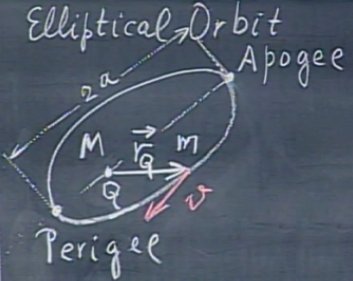
\includegraphics[scale=0.6]{\pIImages/lec22_elliptical_orbit}
\end{center}

Say $M$ here represents the Earth, located an one focus of the ellipse. $m$ is perhaps a satellite or such that orbits the Earth, with velocity $\vec{v}$, with the position vector $\vec{r_Q}$ from Earth.\\
When the satellite is at the closest point to Earth, we say it is at \emph{perigee}. At the farthest point, it is at \emph{apogee}. The distance between apogee and perigee is $2a$, i.e. the major axis of the orbit.

If $M$ instead represented the Sun, and $m$ orbited the Sun instead (where $m$ could be the Earth, or some other planet), we instead call the closest approach \emph{perihelion}, and the farthest point is at \emph{aphelion}. The distance between the two extremes is still $2a$; only the names change.

We can now re-write a few of our equations:

\begin{align}
T^2 &= \frac{4 \pi^2 a^3}{G M}\\
v_{esc} &= \sqrt{\frac{2 M G}{r(t)}} \text{(by setting $E_{tot} = 0$)}\\
E_{total} = K + U &= \frac{1}{2} m v(t)^2 - \frac{m M G}{r(t)} = - \frac{m M G}{2a} = \frac{1}{2} U
\end{align}

The total mechanical energy is still a constant (which is not proved here). Not only is it still constant, but it also has the same value as it would for a circular orbit with the same radius as the semi-major axis of the elliptical one. That is, all we do is replace the $R$ by $a$, and we have the constant energy total.

What is however not constant now is the two energy terms on their own. The kinetic energy now changes, since the orbital speed is no longer constant.\\
The gravitational potential energy also changes with time, since the distance to the Sun is no longer constant.

The escape velocity now also changes with time, though the expression looks about the same as it did for circular orbits, only that the constant radius $R$ has been replaced by the current distance to the sun, $r(t)$.

\begin{center}
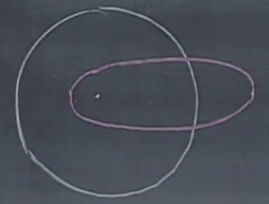
\includegraphics[scale=0.6]{\pIImages/lec22_equivalent_orbits}
\end{center}

These two orbits were drawn to have the same semi-major axis ($R = a$). This means that not only is the total mechanical energy the same for the two, but the time taken to complete one orbit is also exactly the same for either orbit.\\
What about angular momentum? Is it the same for both orbits, and if not, which one has more?

First off, angular momentum is conserved for elliptical orbits. This is clear if you use the same arguments as you do for circular orbits: the only relevant force is the gravitational force; that vector points straight from the planet towards the Sun. The position vector points straight from the Sun towards the planet. Therefore, the torque $\tau_Q = \vec{r_Q} \times \vec{F} = 0$, since the cross product of parallel/anti-parallel vectors is zero. With no external torque, angular momentum must be conserved -- \emph{with respect to the center of the orbit} Q, and not in general!

We can write the angular momentum relative to point $Q$ (the center of orbit) as $L_Q = \vec{r} \times \vec{p}$. However, in the case of the elliptical orbit, the magnitude of both these vectors change in time.  What doesn't change is the angular momentum relative to this point (see above). Because it is conserved, we can calculate the value at any point of the orbit, and if the value is smaller than it would be for a circular orbit of the same mean distance, that must mean the angular momentum is always smaller. (Or the other way around, if it is bigger.)

The answer is that it is smaller. Using the above information, consider a very elongated orbit, with a semi-major axis the same as the circular orbit we compare it to of course, but with a smaller semi-minor axis. Since angular momentum is constant, we can calculate the angular momentum at a point where it is very far from the Sun. Here, the position vector is large, but the velocity vector is small, and the angle between them is also small. This makes the cross product, proportional to the sine of the angle, small.\\
Alternatively, consider the case where the two orbits overlap. For the circular orbit, the position vector and velocity vector are always constant, and always at 90 degree angles.\\
In the case of the elliptical orbit, the position vector is the same (of course, it's the same point), but the velocity vector differs, and makes a smaller angle with the position vector. I find it reasonable that the cross product is then smaller in this case, but I wouldn't call it completely obvious.

Let's now try to find some information about an orbit, given some initial conditions. We are have an object moving at a velocity $v_0$ near the Earth, which makes an angle $\varphi_0$ with the position vector $\vec{r_0}$ from the Earth, at some $t = 0$. Given these details plus the mass $M$ of the Earth, can we find all the details about the orbit, such as: the semi-major axis, the velocity at any given point, the perigee and apogee (closest and furthest distances from the Earth), and so on? The answer is yes, we can.\\
(Needless to say, we can do this for orbits around the Sun, too; the Earth is merely an example.)

\begin{center}
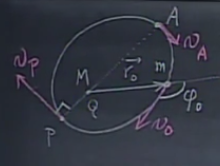
\includegraphics[scale=0.6]{\pIImages/lec22_initial_conditions}
\end{center}

We start out by finding the total mechanical energy, which we can use to find the semi-major axis. One of our equations for elliptical orbits is

\begin{equation}
E_{total} = K + U = \frac{1}{2} m v(t)^2 - \frac{m M G}{r(t)} = - \frac{m M G}{2a} = \frac{1}{2} U
\end{equation}

In this case, we can find the mechanical energy at this instant $t = 0$, since we know everything we need to know in the above equation:

\begin{align}
\frac{1}{2} m v_0^2 - \frac{m M G}{r_0} &= -\frac{m M G}{2a}\\
a \left(v_0^2 - \frac{2 M G}{r_0}\right) &= -M G\\
a &= -\frac{M G r_0}{v_0^2 r_0 - 2 M G}
\end{align}

Since $a$ cannot be negative, the second term in the denominator \emph{must} be greater than the first, so that the signs work out. We can rewrite the equation with this in mind:

\begin{equation}
a = \frac{M G r_0}{2 M G - v_0^2 r_0}
\end{equation}

This only holds for bound orbits. If $E_{tot} > 0$, $a$ must be negative, which makes no physical sense. The equation is simply invalid at in that case.

We can now apply
\begin{equation}
T^2 = \frac{4 \pi^2 a^3}{G M}
\end{equation}

given that we know $a$, so we also know the orbital period at this point.\\
The escape velocity also follows easily, since all you need to know there is $M$ and the distance to he center of that mass $r$.

Next up, we want to find the angular momentum of the orbiting object, relative to the center of the mass $M$ (which we call point Q), as the conservation of angular momentum is helpful for finding some other orbital properties. We can relate the initial angular momentum with the angular momentum at perigee (point P). The distance at perigee is QP, and so we have

\begin{equation}
|L_Q| = m v_0 r_0 \sin \varphi_0 = m v_p (QP)
\end{equation}
The first term is the cross product $(\vec{r_0} \times \vec {v_0}) m$, i.e. the angular momentum as we start out. The second term is the cross product $(\vec{r_p} \times \vec{v_p}) m$, only we call the distance QP instead of $r_p$.

Both $v_p$ and QP are unknown, so we need a second equation. We can find another using the conservation of mechanical energy. At point P, we have

\begin{equation}
\frac{1}{2} m v_p^2 - \frac{m M G}{QP} = - \frac{m M G}{2a}
\end{equation}

Now, as an added bonus, when we solve this, we will get two answers, since this equation is quadratic in $v_p$. One solution will be $v_p$, and the other will be $v_A$. We will also find both QP and QA (the perigee and apogee distances). The reason we find both of these values is rather simple: we have said that the angular momentum is $m v_p (QP)$. There are only two places where the position vector and the velocity vector are exactly perpendicular: at perigee, and at apogee. The equations are equally valid at both points, since the equation doesn't know that we said $v_p$ and QP; it might as well have said $v_A$ and QA, and we would have found the same answers.

The solutions I got were extremely ugly; I'm not sure if they can be simplified further using physics knowledge, but Mathematica can't do any better than this.

\begin{align}
v_p        &= \frac{a G M - \sqrt{a G M \left(a G M- r_0^2 v_0^2 \sin^2 (\varphi_0)\right)}}{a r_0 v_0 \sin (\varphi_0) }\\
\text{QP}  &= a + \sqrt{a\left(a - \frac{r_0^2 v_0^2 \sin^2(\varphi_0)}{G M}\right)}\\
v_A        &= \frac{a G M + \sqrt{a G M \left(a G M- r_0^2 v_0^2 \sin^2 (\varphi_0)\right)}}{a r_0 v_0 \sin (\varphi_0)}\\
\text{QA}  &= a - \frac{\sqrt{a G M(a G M - r_0^2 v_0^2 \sin^2(\varphi_0))}}{G M}
\end{align}

Because the angular momentum $m(\vec{r} \times \vec{v})$ must remain a constant at all times, it must be true that at perigee/apogee when the cross product equals simply $m r v$, the product of the distance and the velocity must be the same in both cases. That is, $m v_p (QP) = m v_A (QA)$. The mass cancels, of course, so we find that $v_p (QP) = v_A (QA)$ must hold.

Apogee is by definition farther from the Earth than perigee, so the speed at apogee must be lower.\\
The difference in speed can be rather enormous, for very elliptical orbits. If apogee is 14 times as far away as perigee is, the speed at perigee will then be 14 times \emph{higher} than the speed at apogee. If this were not the case, angular momentum would not be conserved (relative to the point Q, the only point relative to which it is \emph{ever} conserved).

So in conclusion, by knowing the initial position, velocity (including the direction, i.e. angle between position vector and velocity vector) and the mass of the object we orbit, we can find all the orbital details. This is assuming that the orbital will be elliptical ($a > 0$ when we calculate it, using the first equation). If that is not the case, then there will be no bound orbit, and some of these parameters are meaningless (such as apogee/aphelion, the orbital period, etc). In any case, we can not deal with that using what we have learned \emph{so far}.

\subsection{Change of orbits}

Let's look at a simplified case of a change in orbit. We begin in a fully circular orbit, and then fire a rocket exactly tangentially to the orbit.\\
Say we begin at the ``top'' of the orbit (in a diagram), at point X. We fire the rocket a very short amount of time, so that we can consider that it is still at X afterwards. The speed will increase, so the kinetic energy will increase, and the total mechanical energy will increase (we have not moved away, so gravitational potential energy must be the same, assuming our mass has not changed).

Because our velocity is now greater, and we are at a certain distance $R$ from the planet (or star, or whatever), our velocity is no longer the correct velocity for a circular orbit at this distance. Instead, we go into an elliptical orbit, where $a > R$. The total mechanical energy has increased, which means $a$ must increase; total mechanical energy is $-\frac{m M G}{2 a}$, and for mechanical energy to increase, that number must become less negative. A larger $a$ does exactly that. Via the relationship in $T^2$, this also implies that the period of this new orbit is greater than the old period, despite the increase in speed.

\begin{center}
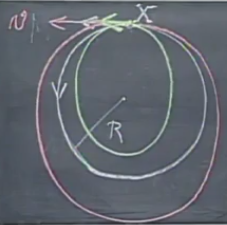
\includegraphics[scale=0.6]{\pIImages/lec22_orbit_change}
\end{center}

In this graphic, the original orbit (fully circular) is in white. We are orbiting counterclockwise, as seen here.\\
For the red orbit, we have increased our tangential velocity, and so the orbit grows, and becomes elliptical. $E_{tot} > E_{tot,circular}$, and so the semi-major axis is greater than the original radius, and the period is greater than the original, since $T^2 \propto a^3$.

For the green orbit, we instead fired our rocket exactly opposite to our velocity, so that we slowed down, and lost kinetic energy, and also lost total mechanical energy.\\
In that case, $a < R$, and the period goes down.\\
Out of context, it sounds rather crazy: you go around faster by braking! Of course, you also travel a shorter distance per period, so there's nothing particularly crazy about it.

The rest of this lecture will focus on a ``practical'' (fun, at least) example of this; perhaps we can call it several examples, even.

Two astronauts, Peter and Mary, are in orbit around the Earth. They are both moving at the same speed, and are at the same distance from Earth, sharing a circular orbit. They are not moving along it together, however. Peter is at one place along this circular orbit, point X, while Mary is at a point M, a distance further along. We can specify this separation as a fraction of the circumference $2 \pi R$ of the orbit, using $f$ as the fraction. The distance between the two is then $f\ 2 \pi R$. The rest of the orbit must then be $(1-f) 2 \pi R$, which is the amount of distance Mary must move before she ends up at point X (which she recently passed).

\begin{center}
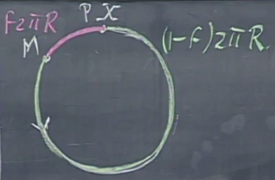
\includegraphics[scale=0.6]{\pIImages/lec22_peter_mary_orbit}
\end{center}

Say the radius of this shared orbit is $R = 7000$ km ($\SI{7e6}{m}$), and $f = 0.05$, which makes the separation between the two about 2200 km. (The actual separation as a straight line is smaller, but we don't really care about that.)\\
Given these parameters, there is a only one possible circular orbit: the radius of the orbit puts a demand on the velocity and period of the orbit. This velocity is about 7.55 km/s, and the period is about 97 minutes.

If we round things off a bit, it then takes $f T \approx 5$ minutes to travel the distance that exists between Peter and Mary. This means it takes 92 minutes for Mary to get to the point where Peter is currently. (Needless to say, Peter will no longer be there when she gets there.)

Now, here is the problem: Mary forgot her lunch. She radius Peter, who says not to worry; he will throw her a ham sandwich. The question is: how will he do this, so that Mary can catch it? Perhaps the simplest way is to throw the sandwich such that its new orbit brings it to point X, where Mary will be, in exactly the 92 minutes required, so that Mary and the sandwich meets at that point.

Here comes the counter-intuitive part (at least to me): if Peter throws the sandwich forward, it will come back to point X \emph{later} than Mary. The faster he throws it, the longer it will take.\\
The reason is that by throwing it, he is doing exactly what we did with the rocket earlier on. The sandwich will move into an elliptical orbit, with $a > R$. Since $T \propto a^{3/2}$, this orbit has a longer period than Peter's, and so the sandwich will take a longer time to get into place for Mary's move past point X.

Instead, he needs to throw it \emph{backwards}, and \emph{reduce} its orbital speed. That way, it will move into a smaller orbit, with a smaller period, and come back to point X faster, by having moved a smaller distance.

What we need is that the orbital period of the sandwich $T_s$ is less than Mary's period $T_a$ (a for astronaut), such that $T_s = (1 - f) T_a$. $T_a$ is 97 minutes, and the orbit we want should be 92 minutes. $1 - f = 0.95$, and $0.95 \times 97$ minutes is about 92 minutes. (Keep in mind that all of these numbers for the period are rounded approximations; the actual period $T_s$ will be exactly right.)

Doing the actual math, we need the sandwich's orbit to be $(1-f)$ times the astronauts' orbit, as mentioned, which using Kepler's third law is

\begin{equation}
\sqrt{\frac{4 \pi^2 a^3}{G M}} = (1-f) \sqrt{\frac{4 \pi^2 R^3}{G M}}
\end{equation}
\begin{align}
\sqrt{a^3} &= (1-f) \sqrt{R^3}\\
a &= (1-f)^{2/3} R
\end{align}

So knowing only the radius of their orbit and how far they are apart along that orbit (as measured by a fraction $f$ of the total circumference), we can find what the radius of the sandwich, $a$, must be.\\
Knowing $a$, the semi-major axis of the sandwich's orbit, we can now calculate what velocity it must have, using the equation for total mechanical energy.

\begin{equation}
\frac{1}{2} m v_s^2 - \frac{m M G}{R} = -\frac{m M G}{2a}
\end{equation}

On the right-hand side, we have the current kinetic energy of the sandwich (after the throw), and its current gravitation potential energy. An instant after the throw, we can still consider it to be at point X, so it is still a distance $R$ from the planet. The right-hand side of the equation must always hold for elliptical (and thus also circular) orbits: the total mechanical energy is always $\displaystyle \frac{1}{2} U$.

We can solve this for $v_s$, now that we know everything else. $m$ cancels, as always, and in the end, we find

\begin{align}
\frac{1}{2} v_s^2 - \frac{2 M G}{R} = -\frac{M G}{a}\\
v_s^2 = \frac{2 M G}{R} - \frac{M G}{a}\\
v_s^2 = \frac{2 M G}{R} - \frac{M G}{a}\\
v_s = \sqrt{\frac{G M (2 a - R)}{a R}}
\end{align}

In terms of $R$ (since we know $a$), this is also

\begin{equation}
v_s = \frac{\sqrt{(2(1-f)^{2/3} - 1) G M R}}{(1 - f)^{1/3} R}
\end{equation}

In terms of numbers, we have $a = 6765$ km -- smaller than $R$, which it must be; $v_s = 7.42$ (though closer to 7.43) km/s.\\
The speed of the sandwich \emph{relative to Peter} is what matters to hit, though: he doesn't need to throw it at over 7 km/s! He just needs to throw it so that its final velocity $v_s$ is that value, but most will come from his current orbital speed $v_a$.

The speed he needs to throw it at is $v_s - v_a = 0.13$ km/s. Note how $v_s < v_a$ -- it moves in a smaller orbit, but therefore also moves at a lower speed.

So in order for Mary to catch it the \emph{first time she passes point X again}, he must throw the sandwich \emph{backwards} (towards the clockwise direction), slowing its speed and reducing its total energy, even though he can see Mary currently in front of him!

Unfortunately, 130 m/s is a bit much for a person to throw a sandwich. We can find a different solution, where the sandwich moves around the Earth multiple times, and possibly where Mary does too.\\
Mathematically, we can have Mary pass the point $n_a$ times ($n$ for number of times, $a$ for astronaut), and the sandwich $n_s$ times. Both numbers need to be integers, of course.

We now find

\begin{equation}
a = R \left(\frac{n_a - f}{n_s}\right)^{2/3}
\end{equation}

as the semi-major axis for the sandwich's orbit. If $n_a = n_s = 1$, the equation reduces down to what we had previously.\\
Not all combinations of integers will work, however.

For $n_a = 1$ and $n_s = 3$, such that the sandwich should make three orbits in the same time Mary completes her one orbit, the result is invalid.\\
For these numbers, we find $a = 3252$ km (versus $R = 7000$ km).\\
$2a < R$, which is not allowed; the reason why can be seen in the equation for $v_s$. If we the $a$ value in, we find an imaginary answer (complex, but the real part is 0).\\
As $a$ approaches $R/2$, $v_s$ goes to zero. There is the possibility where he throws it at exactly his orbital speed, in which case it will stand still relative to the Earth, and fall straight down. What if he throws it ever faster? In that case, there is clearly no longer a counterclockwise orbit, which has been our assumption all along.

The final part of the lecture shows a computer simulation of this scenario, including a few cases not mentioned in this text.

\section{Lecture 23: Doppler effect, binary stars, neutron stars and black holes}

The speed of sound, in air, is about 340 m/s, at roughly room temperature. The range is something like 306 m/s near $-40$ degrees Celcius (which also equals $-40$ degrees Fahrenheit) and 360 m/s at 50 degrees Celcius ($122^\circ$ F), which hopefully covers most temperatures we encounter.

When a person speaks, his/her vocal cords oscillate at a certain frequency, which causes a pressure wave in the air to move towards you, at the speed of sound. Your eardrums then oscillate at the this same frequency, which your brain can interpret as a certain pitch.

If the sound transmitter is moving away or towards the receiver, the perceived sound frequency will change. The faster the transmitter is approaching you, the higher the perceived frequency, and vice versa. If the transmitter is moving away from you at the speed of sound, you will hear exactly half the original frequency.\\
That is, if we use prime notation for the perceived frequency and $f$ for the original frequency,

\begin{align}
f' &> f \text{ (when sound source is approaching you)}\\
f' &< f \text{ (when sound source is moving away from you)}
\end{align}

More quantitatively, when a source source is moving towards you, but you are sitting still, the frequency you perceive is

\begin{equation}
f' = f(1 + \frac{v}{v_s} \cos \theta)
\end{equation}

where $v_s$ is the speed of sound, and $v \cos \theta$ is the radial speed, i.e. the speed at which the transmitter is moving towards you. If the transmitter is moving quickly, but at a 90 degree angle to you, you don't hear any shift in the frequency.\\
If the transmitter is moving \emph{away} from you, the frequency you perceive goes down, which this equation also captures (for negative values of $\cos \theta$).

The professor demonstrates this by using a 4000 Hz tuning fork, moving it back and forth towards and away from the students. If this is done at roughly 1 m/s, the pitch will change with $\pm 0.3$\% which is $\pm 12$ Hz. This difference is clearly audible, including in the recorded video of this lecture.

This effect of frequency change is known as the \emph{Doppler effect}. It is the reason behind the familiar scenario where the pitch of an ambulance/police car/fire truck's siren changes as it travels past you.\\
When the sound transmitter is moving away from you, the pitch you hear is lower than the pitch that is actually transmitted at the source. If the transmitter is coming towards you, the pitch instead increases.

Note that the case of a stationary transmitter and a receiver moving away is \emph{not} equal to the case of a stationary receiver where the transmitter is moving away!

If the transmitter is stationary, and is creating sound waves with a frequency of say 440 Hz (the standard tuning in all modern music is to the A440 note), and the receiver moves away at the speed of sound, then there will be no sound heard at all - the receiver (just barely) outruns the sound waves entirely!

On the other hand, if the \emph{transmitter} is moving away at the speed of sound, while the receiver is stationary, the result is that the perceived frequency is cut in half to 220 Hz.\\
So we still hear the sound, in this case. If you find that nonintuitive, think about it a bit more - it's very clear that while the transmitter moves, the waves will still reach you as they always travel at 340 m/s in your direction. The transmitter may be moving in a direction away from you, but the sound waves don't travel along with the transmitter, but towards you (and it all other directions, too, assuming an omnidirectional speaker).

Let's now consider the case where the transmitter is moving around in a circle. Now, the perceived frequency, assuming the receiver is still stationary, will vary sinusoidally around the base frequency of $f$ that the transmitter is sending out.

\begin{center}
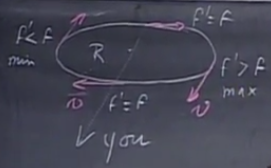
\includegraphics[scale=0.6]{\pIImages/lec23_doppler}
\end{center}

When the source is moving straight towards you, $f'$ is at a maximum; the opposite is true when it is moving straight away from you. At the other two extremes, when it is at 90 degree angles, $f' = f$, and so there is no change in frequency at those times. In between, as you might expect, there is a gradual change between these extremes.

If we, as the receiver, plotted the frequency we heard as a function of time, we would get something like this:

\begin{center}
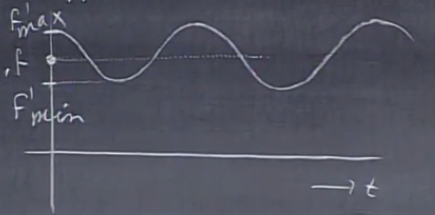
\includegraphics[scale=0.5]{\pIImages/lec23_doppler_circle}
\end{center}

If we have this curve, we can calculate an impressive number of things. First, we know ${f'}_{max}$ and $f$, which means we can calculate the velocity of the transmitter.\\
We can also measure the period of one rotation, by measuring the time from one peak to the next (or one valley to the next, etc). Knowing that, we can find the radius $R$ of the circle the transmitter is moving in:

\begin{align}
\frac{2 \pi R}{T} = v_{tr}\\
R = \frac{T v_{tr}}{2 \pi}
\end{align}

So from simply listening to/measuring the sound over time, we can calculate these three things, rather easily.

How do we intuitively explain the Doppler effect? It is actually quite simple, but is best shown using animated graphics, which I can't really use here. I suggest looking it up online. Wikipedia has some very nice animated figures, for example.\\
In short, when moving towards a transmitter (or the transmitter is moving towards you), the wave fronts become ``compressed'', and the wavelength becomes shorter (meaning that for sound, the pitch increases; for light, it becomes \emph{blueshifted}; more on that soon). When the distance between is increasing, the wave fronts become separated from each other, and the wavelength becomes longer (sound: lower pitch; light: ``redder'' color, or redshift).

\subsection{The Doppler effect and electromagnetic waves/light}

Let's look more at the Doppler effect in light (and other EM radiation).

\begin{center}
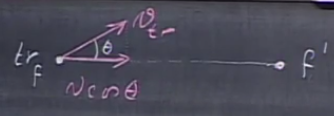
\includegraphics[scale=0.6]{\pIImages/lec23_doppler_em}
\end{center}

The equation given in lecture, which is only valid for $v \ll c$, i.e. when the relative velocity between transmitter and receiver is much smaller than the speed of light, is:

\begin{equation}
f' = f (1 + \frac{v}{c} \cos \theta)
\end{equation}

In calculating the Doppler shift due to some relative motion, only the radial component, meaning the part of the velocity that is directly towards or from you, matters. Therefore, we take the cosine of the angle of the velocity vector. Note that the radial component is given as $v \cos \theta$, rather than $v_{tr} \cos \theta$ (tr for transmitter); the index was dropped as it does not matter whether the transmitter or the receiver is moving, or both. (It is even really a meaningless question in relativity; moving relative to what reference frame?)\\
There is however something known as the transverse Doppler shift, which occurs even at 90 degree angle. I'm not sure when this matters, but it is not mentioned in the lecture, at all, so I suppose it is less important in most cases.

Much of the idea behind special relativity, as the name implies, is that motion is relative. There is no such thing as an absolute reference frame, and therefore, there is only one term of velocity in the equation. It is meaningless to ask whether person A is moving towards person B, or person B is moving towards person A. What we can say is that they are approaching each other.\\
It does however, of course, matter whether the two are approaching or receding from each other.

In this equation, if $\theta < \ang{90}$, $f' > f$ since the cosine term will contribute to increasing $f'$. If $\theta > \ang{90}$, the cosine will be negative, and $f' < f$. At 90 degree angles, as mentioned, this equation will tell you that there is zero Doppler shift. And again, this only holds if $v \ll c$, i.e. $\displaystyle \frac{v}{c} \ll 1$.

All electromagnetic radiation, whether it is visible light, gamma rays, microwaves, radio waves etc., has a frequency associated with it. Anything with a frequency of oscillation also has a \emph{period} of oscillation, with the simple relationship that $T = 1/f$.\\
How far does EM radiation travel in a time T? Well, it travels at the velocity $c$, the speed of light ($c \approx \SI{3e8}{m/s}$, to within 0.07\%). That means the distance traveled is $\lambda = c T$, where $\lambda$ (lowercase Greek letter lambda) is the symbol we use to denote \emph{wavelength}.

\begin{equation}
\lambda = c T = \frac{c}{f}
\end{equation}

For example, if $T = \SI{2e-15}{s}$, $\lambda = \SI{6e7}{m}$, which is the about wavelength of red light.\\
If instead $T = \SI{1.3e-15}{s}$, $\lambda = \SI{3.9e7}{m}$, which we perceive as blue light.

In optical astronomy, we can only measure the wavelength of light -- not frequency or period -- so we can rewrite some of our equations to better accommodate this. We can of course calculate frequency, so that

\begin{align}
f  &= \frac{c}{\lambda}\\
f' &= \frac{c}{\lambda'}
\end{align}

With that in mind, we can find

\begin{equation}
\lambda' = \lambda(1 - \frac{v}{c} \cos \theta)
\end{equation}

What was a plus sign in the previous equation of this sort is now a minus sign. Also, keep in mind that this equation also has the restriction that $v \ll c$.

Since frequency is inversely proportional to wavelength, $\lambda' < \lambda$ if the object is approaching you ($\theta < \ang{90}$). This is known as \emph{blueshift}. The name comes from the fact that all radiation becomes more energetic (higher frequency/smaller wavelength), which causes visible light to shift towards the blue end of the spectrum. (EM radiation that is already more energetic than blue/violet light becomes even more energetic, and therefore shifts even further away from the visible spectrum, towards the gamma rays.)

Similarly, if the object is moving away from you, $\theta > \ang{90}$ and $\lambda' > \lambda$. A longer wavelength means less energy, and this is known as \emph{redshift}. Here, all light becomes less energetic and ``stretched out'', which shifts visible light (and all more energetic light) towards the red end of the spectrum. Light that was already lower energy (microwaves, radio waves) lose further energy and shift further away from the red (and further from visible light altogether).

In case the above is written in a confusing manner: blueshift is called as such because visible light is shifted towards the blue. \emph{All} light, regardless of frequency/wavelength becomes \emph{more} energetic when blueshifted. Conversely, redshift is called as such because visible light is shifted towards the red, and all light, regardless of frequency/wavelength becomes \emph{less} energetic when redshifted.

\subsection{Emission and absorption spectra}

We can look at the light spectra of stars, and look at the intensity of the light as a function of wavelength. When plotting that, we will not see a continuous distribution, as we might expect. Instead, we see a mostly smooth curve, with some sharp spikes downwards. That is, light intensity is sharply reduced for certain wavelengths.\\
We call these \emph{absorption lines}. Each absorption line is due to some element present in the atmosphere of the star. Through the process of figuring out which elements and isotopes cause which absorption lines here on Earth, we can use the lines to figure out which elements are present in the star.

Here is an example of \emph{emission lines}, in this case of hydrogen:

%TODO: add images
%\begin{center}
%\includegraphics[scale=0.75]{\pIImages/lec23_hydrogen_emission}
%\end{center}

The red line on the right is known as H$\alpha$ (hydrogen alpha), and is a very well-known spectral line. Telescopes are often fitted with H$\alpha$ filters for viewing the Sun.\\
Emission lines are the \emph{opposite} of absorption lines. In this case, we use a lamp or such that excites hydrogen, which then only produces light in discrete steps, for quantum mechanical reasons.

If you have ever seen street lightning that makes everything appear yellow, those lamps were most likely sodium-vapor lamps. These lamps, especially the low-pressure type, are almost entirely monochromatic, and essentially only emit light at two wavelengths, about 589.0 and 589.6 nm -- both of which are yellow.\\
Since vision relies on having light reflect off things and enter our eyes, in the presence of only such light, it is impossible to see colors other than yellow. Objects that completely absorb yellow will become dark. For this reason, the amount of different wavelengths a lamp emits is a common measure of its perceived quality (see color rendering index aka color rendition index, CRI).

As mentioned, absorption lines are the opposite of this. Here is an example of absorption lines:

%TODO: add images
%\begin{center}
%\includegraphics[scale=0.75]{\pIImages/lec23_absorption_spectrum}
%\end{center}

The letters refer to labels of Fraunhofer lines, a set of spectral lines named after (and identified by) German physicist Joseph van Fraunhofer, in the early 1800s. The sodium lines above can be seen as D1 and D2 in the yellow-orangeish part of the spectrum.

The now-well known element helium was first discovered in Sun, as an absorption line that could not be reproduced in the lab here on the Earth was identified. The element was named  helium, after Helios, the Greek Sun god.

What is now interesting, and extremely useful, is that the relative spacing of these lines stays constant. If a star is moving (radially) relative to us, the light will be either redshifted (if it moves away) or blueshifted (if it moves towards us), but since \emph{the entire spectrum} will be shifted, we can still identify what elements are present via their distinct patterns and spacings.\\
This means that we can not only look at a star and figure out what it is made of, we can also calculate its velocity relative to us!

For example, if $\lambda'/\lambda = 1.000333$, according to the equation we found earlier, the star is moving at $-0.000333 c$ (radially), where the minus sign signifies that it moves away from us. That is, $v \cos \theta = -0.000333c = -100$ km/second. Note that since $\lambda' > \lambda$, the light from the object has been redshifted. Also note that we cannot say what $v$ is using this information, only what the radial component is -- i.e. how fast it moves towards us, or from us.

As a very quick aside, this is how police ``radar guns'', which can measure the speed of cars, work. They reflect radar waves of a known frequency/wavelength off cars, and measure the wavelength of the returning waves. The radial velocity of the car can then be calculated, using the measured Doppler shift.

\subsubsection{Spectra of binary stars}

Binary stars, pairs or stars that orbit each other, are extremely common. The lecture states that half of the stars in the sky are binaries. I'm not sure if that refers to visible stars, in which case I would guess nothing has changed, but it \emph{may} (with emphasis, indeed) be that science's view has shifted, and that most stars overall are in fact not binaries, from recent (post-lecture recording) news articles.

When binary stars orbit each other (or rather their shared center of mass), we can measure the Doppler shift they exhibit. While orbiting, they will be going towards us, at right angles, from us, etc. just as with the sound source moving in a circle we looked at earlier.\\
This is only possible to see if we are in the plane of their orbit, however. If we are looking at the system from ``above'', the radial component of the velocity between the stars and us will be constant despite the orbit, as they will not move any closer to us or further from us due to the orbit.

Just as in the case with sound, we can measure and calculate the period of this shift, and therefore calculate their velocities, the orbital period, and the orbital speed.

\begin{center}
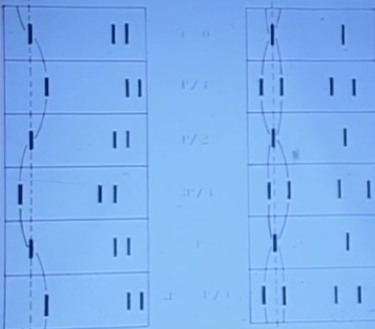
\includegraphics[scale=0.75]{\pIImages/lec23_binary_spectrum}
\end{center}

Above is an illustration on the Doppler shift in the spectrum of a binary star system. On the left, we have the case where we can only see one of the two stars. As time passes, we see the spectral lines shift left and right (as time passes, downwards in the picture) in unison.\\
On the right, we have the case where we can see both stars. In this simplified case, we only show the same two spectral lines. In this case, when we see the spectral lines of one star redshifting, the other will be blueshifted, and vice versa, in the case that one is moving from you, and the other towards you. This means that one set of lines will move towards the left, as pictured, while the other moves towards the right, doubling the number of spectral lines we observe.

As mentioned previously, based on this data, we can then calculate the orbital radius, velocity in orbit, and the (shared) period of the two stars' orbits.

Let's now consider a binary system. They orbit their common center of mass, and are in different circular orbits, of radii $r_1$ and $r_2$, respectively. The stars have masses $m_1$ and $m_2$, and velocities $v_1$ and $v_2$.

\begin{center}
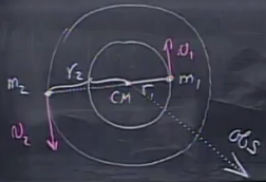
\includegraphics[scale=0.75]{\pIImages/lec23_binary_orbit}
\end{center}

Via the definition of center of mass, $m_1 r_1 = m_2 r_2$.\\
We, as an observer, are somewhere in the plane of this orbit, but far away from it.

Via Kepler's third law, which we have seen before,

\begin{equation}
T^2 = \frac{4 \pi^2 (r_1 + r_2)^3}{G (m_1 + m_2)}
\end{equation}

If we measure the Doppler shift of star 1, we can find its period $T$, its velocity $v_1$, and its orbital radius $r_1$. We make a similar measurement for the second star, and find $T$, $v_2$ and $r_2$.\\
Because we then know $r_1$ and $r_2$, we obviously also know $r_1 + r_2$. We also know $T$. Using this information, using the equation above, we can find $m_1 + m_2$!\\
Not only that, but we also know that $m_1 r_1 = m_2 r_2$, so we can find $m_1$ and $m_2$ on their own, too, given that we have two equations relating the masses and orbital radii.

Using nothing but two Doppler shift measurements and some calculations, we can find the mass of each star, the radius of their orbit, how fast they move in that orbit, and the time it takes the pair to orbit once. Incredible.\\
If we are not in the plane of the orbit, however, we must have extra information: we need to know the angle $\theta$ we make with the orbital plane. We will only measure the radial components of the stars' velocities, and so only by knowing $\theta$ can we make any calculations on their actual velocities in orbit.

\subsection{X-ray binaries}

Let's now have a look at a special case of binary stars. In an X-ray binary system, we have two different types of stars: one large, relatively normal star, not too unlike our Sun.\\
The other star is a neutron star, or a black hole (or in some cases, a white dwarf). Let's assume it is a neutron star for this discussion.

Consider what happens if the two have the same mass. There will then be a point, right in the middle between them, where the gravitational pull is the same in both directions. We call this the inner Lagrangian point. If instead this point is inside the larger star, matter will fall from that star onto the neutron star, since the gravitational pull for all matter outside that point will have a stronger gravitational force towards the neutron star.

\begin{center}
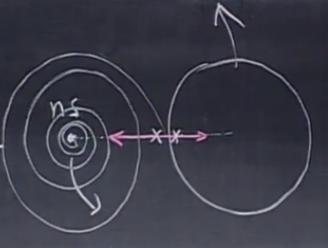
\includegraphics[scale=0.6]{\pIImages/lec23_xray_binary}
\end{center}

Here, we see the larger star as the ring to the right, with the arrow indicating how it is orbiting. The neutron star is the small dot at the center of the spiral; the spiral is made up by the infalling matter, and is called the \emph{accretion disk}. Matter cannot fall radially inwards towards the neutron star, because of the fact that the two are orbiting each other (or their common center of mass, rather).

The neutron star is also called the accretor, while the larger star is known as the donor.

Consider now a small amount of matter $m$ that is released far from the neutron star. Technically, ``far'' means infinitely far away, but the answers we find are almost identical for reasonably small distances (starting out at just 1000 km from the neutron star instead of infinitely far away, the impact velocity is 99.5\% of what it is if you begin at infinity, so the impact energy is about 99\%).

We know that total mechanical energy is conserved, so the velocity of the piece that hits can be found by considering its energy as it hits, and far away, where $U = 0$ and also $K_e = 0$ (if we let it go with zero speed):

\begin{equation}
\frac{1}{2} m v^2 - \frac{m M_{ns} G}{R_{ns}} = 0
\end{equation}
\begin{equation}
v = \sqrt{\frac{2 M_{ns} G}{R_{ns}}}
\end{equation}

The kinetic energy as it hits is clearly $\displaystyle \frac{1}{2} m v^2$, where $v$ is the above impact velocity:

\begin{equation}
K_{impact} = \frac{m M_{ns} G}{R_{ns}}
\end{equation}

For $m = 10$ grams (0.01 kg), $M_{ns} = 1.5$ solar masses ($1.5 \times \SI{2e30}{kg}$) and $R_{ns} = 10$ km, we find $K_{impact} = \SI{2e14}{J}$. The impact velocity is $\SI{2e8}{m/s}$ -- ignoring relativistic effects. Keep in mind that this is for a \emph{10 gram} object! This energy output is comparable to that of the atomic bombs used in world war 2 -- all because of a 10 gram object being released from being (relatively) close to a neutron star.

There are hundreds of such systems (that are known) in our galaxy.\\
The mass transfer rate in such systems is something along the lines of $\displaystyle \frac{dm}{dt} = 10^{14}$ kg/s -- which is, of course, a rather insane number. Now, consider how much energy was released from the tiny 10 gram mass falling onto the neutron star! Here, we have $10^{16}$ times more mass \emph{per second}.\\
All in all, this gives an energy rate (power) of about \SI{2e30}{W}, about 5000 times the power output of our Sun.

Because of this enormous energy release, the temperature of the neutron star is about 10 million Kelvin. At such high temperatures, most of the EM radiation emitted is in X-rays.\\
We humans have body temperatures of about 300 K; at that temperature, we emit infrared radiation -- heat. We cannot see this radiation, but we can feel it as heat. An object at 3000 K would glow red-orange due to its temperature. At 3 million K (or degrees Celcius, which are practically the same; the difference is less than 300 K), X-rays begin to matter.

As the matter falls in, it is usually highly ionized, due to the gravitational potential energy released. Highly ionized material has electric charge, which can only reach the neutron star at certain points. The reason is that neutron stars have extremely strong magnetic fields (in particular, one sub-class called magnetars are thought to be the most strongly magnetic objects in the universe), and the movement of charged particles is affected by magnetic fields. They will tend to follow the magnetic field lines, and enter the neutron star near the two magnetic poles.

These two poles then turn into ``hot spots'', and most matter will fall in a relatively small area -- especially considering that the neutron star is very small to begin with.\\
If the axis of rotation doesn't coincide with these hot spots, we can get the effect where it rotates such that the ``jets'' created by the infalling matter appear to pulsate at us, creating an X-ray pulsar.\\
(Consider the case where it rotates around an axis that goes through its north and south (geographic) poles, while the magnetic field is perpendicular to this.)

The timing of these pulses is, as mentioned a few lectures back, extremely precise. However, now that we have a binary system, we can end up with the scenario where the neutron star is coming towards us, and then moving away from us, during an orbit (again assuming we are in the plane of the orbit). The are a bit like a clock; as it is coming towards us, due to Doppler shift, the ``ticks'' come a little closer together. As it moves away, they are a little further apart. So by timing these pulses, we can measure the Doppler shift of the neutron star, and then as earlier find the orbital radius, period and velocity of the neutron star.

If we combine that X-ray observation with an optical observation of the donor star, we see the Doppler shift in the absorption lines due to its orbit, and so we can calculate from that the donor star's orbital radius, orbital velocity and period.\\
As before, with this information, we can now also calculate the individual masses of the two stars.

In addition to what we have discussed so far, there may also be a change in activity on a longer time scale, of days rather than milliseconds or seconds.\\
If we are indeed in the plane of the orbit, then there will be times where the neutron star passes behind the donor -- and the donor then absorbs the X-ray emissions from the neutron star. This will cause periods where the X-ray activity appears to cease, until this X-ray eclipse is over.\\
This also means that we get a second, independent measurement of the orbital period.

\subsection{Chandrasekhar limit, black holes}

Of all the X-ray binaries measured so far, almost all of the neutron stars have a mass very close to 1.4 solar masses, for good reasons.\\
Indian-American physicist Chandrasekhar calculated in 1930, at the age of 19, that a white dwarf star could not exist if its mass was greater than about 1.4 solar masses. The reason lies in quantum mechanics (above that mass, the gravitational force wins over the electron degeneracy pressure, so that the star collapses -- not that I personally truly know what this means yet). This limit is known as the Chandrasekhar limit; the currently accepted value is about 1.44 solar masses.

So imagine a white dwarf, with a radius about 10 000 km. If we keep adding mass to it, by the time it reaches the Chandrasekhar limit, can collapse down into a neutron star, in a type Ia supernova.

If we instead imagine adding mass to a neutron star, by the time it reaches a mass of approximately 1.5-3 solar masses, it can yet again collapse, in this case into a black hole. This limit is known as the Tolman-Oppenheimer-Volkoff limit (or TOV limit). Similarly to the white dwarf case, a neutron star with a mass under the TOV limit is stable due to the equilibrium between two pressures, this time between the gravitational force and the \emph{neutron} degeneracy pressure.\\
As a sidenote, it is possible that other types of ultra-dense stars exist, such as quark stars. There is not yet any definite proof one way or the other, but they remain a theoretical possibility.\\
For now, let us assume that the ``next step'' from a neutron star is a black hole, and that there exists nothing in between.

What is, then, a black hole?\\
Classically, a black hole is a point mass -- it has no radius in itself. Black hole masses vary by extreme amounts for different types; it is thought that there are types from a few (3-10) solar masses, to ones with a mass of \emph{billions} of solar masses: supermassive black holes. It is also thought that most, if not all galaxies contain a supermassive black hole at their center.

A black hole does have one radius that is useful to talk about: the radius of its \emph{event horizon}. We know how to calculate escape velocities:

\begin{equation}
v = \sqrt{\frac{2 M G}{R}}
\end{equation}

As $M$ grows, there is a point that for a certain distance $R$ away, the escape velocity is the speed of light $c$. Setting the two equal, that radius is

\begin{align}
\sqrt{\frac{2 M G}{R}} &= c\\
R &= \frac{2 M G}{c^2}
\end{align}

At all points inside this radius, the escape velocity is greater than the speed of light. In other words, nothing -- not even light -- can escape, thus the term black hole. It is theoretically possible to escape from all points outside this radius, but it clearly becomes increasingly hard, the closer you come.

This radius is known as the Schwarzchild radius. All black holes have an associated Schwarzchild radius, found using the above formula. We can also use the formula to calculate into how tiny space we would need to compress a mass $M$ for it to become a black hole. Earth's Schwarzchild radius is a bit less than 1 centimeter, which says something about the insane density of black holes (even if they are not truly point masses)!

As a side note, black holes are not magical: there is a common misconception that they are the ``vacuum cleaners'' of the universe, and that they suck in everything around them. While this is true in a sense -- they do have an extremely strong gravitational pull -- they do not have any more of a pull than any other object of a similar mass.\\
If our Sun was magically replaced by a black hole \emph{of the same mass as the Sun}, all orbits in the solar system would remain unchanged. We would still die due to the lack of sunlight, but that's a different story!

Since nothing, including light (of any wavelength) can escape a black hole, how can we still observe them? In fact, \emph{can} we observe them?\\
The answer is that yes, we can. Matter in the accretion disk, that is still falling in and is still \emph{outside} the event horizon, can be observed with no contradictions. Such matter can be extremely hot, due to the release of gravitational potential energy while falling in, plus frictional forces. It can be and often is hot enough to emit X-rays.

Black holes never pulsate, as they have no surface, so you cannot have the two jets rotating around. This also implies that we cannot measure the Doppler shift of the black hole. We can measure the Doppler shift of the donor star, however. If we can also estimate the donor's mass, we can find the black hole's/accretor's mass from knowing that.

Cygnus X-1 is a famous case. It was discovered in the early 1970s. It is an X-ray binary, with an orbital period of 5.6 days. By looking at the absorption lines, astronomers estimated the donor's mass to be about 30 solar masses. (Note that this is different from what we have discussed, where we need measurements of both to \emph{calculate} the masses.)\\
The mass of the accretor must then be about 15 solar masses. Given that this is a very compact object (given that it emits X-rays), and it is clearly much more massive than $\approx 3$ solar masses, it is concluded that the object most likely is a black hole.

Since then, many other X-ray binaries have been discovered, where the accretor is thought to be a black hole.

\section{Lecture 24: Rolling motion, gyroscopes}

First out this week is rolling motion; specifically, the case where there is no slipping or skipping, which we call \emph{pure roll}.

Say we have a cylinder that is in rolling motion. It rotates with angular velocity $\omega$, while its center of mass is moving in a straight line. Say the radius of the cylinder is $R$.\\
Once it has made a complete rotation about its axis, if the distance it has moved relative to the surface below is $2 \pi R$, we call that pure roll.\\
When this is the case, the velocity $v_Q$ of the center point Q, is always the same as the tangential velocity $v_c$ about the circumference. That is, $v_Q = \omega R$ for pure roll. ($v_C = \omega R$ always holds, of course.)

If there is no friction with the surface below, we can imagine both that the cylinder might roll and roll without actually moving anywhere, and the opposite situation where it slides without rolling. In either case, then, we certainly don't have pure roll.\\
Let's now try to apply this in practice. There are no new physics here; as long as we have pure roll, we can analyze it without too much trouble.

Consider a cylindrical object on an incline of angle $\beta$. We want to calculate the acceleration of the cylinder, as it rolls down this slope with pure roll.\\
The cylinder has a mass $M$, radius $R$ and a length $\ell$.

Given two cylinders, both solid, both having the same mass and length, but differing in radii, which will accelerate faster / reach the bottom of the slope faster?\\
My semi-intuitive answer was that they both accelerate at the same rate. Considering $F = ma$ of the center of mass naively (considering only $m g \sin \beta$, the down-slope gravity), neither should win. Considering $\tau = I \alpha$ around the center, the torque is due to friction acting upwards; the larger cylinder has a larger moment of inertia (same mass, larger $R$), but it also gains a higher torque due to friction creating a torque along that longer $R$.\\
In the end, I figured the effects cancel, and $\alpha$ and $a$ are the same.

Let's look at the analytical answer. First, here is the situation will all the forces and such drawn:

\begin{center}
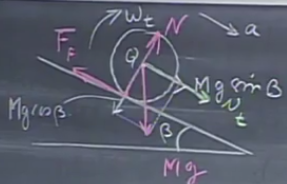
\includegraphics[scale=0.75]{\pIImages/lec24_cylinder_roll}
\end{center}

For pure roll, we can say that the velocity of the center, point Q, must equal the tangential velocity:

\begin{equation}
v_Q = \omega R
\end{equation}

If we take the time derivative of this, we find

\begin{equation}
a_Q = \alpha R
\end{equation}

$a_Q = a$ is then the linear acceleration of the cylinder down the slope.\\
Next, we look at torque. The normal force $M g$ (since there is no acceleration in the $y$ direction, if we set $y$ perpendicular to the slope, $N = F_{gravity}$) and gravity both act through the point Q, so they cannot cause any torque. ($\vec{r}$ in the cross product $\vec{r} \times \vec{F}$ is zero, so the cross product is zero.)

The only force that does cause torque is the frictional force $F_f$, which acts perpendicularly to the center point Q. Therefore, the torque about point Q is simply $\tau_Q = R F_f$.\\
The torque must be equal to $I_Q \alpha$; Newton's second law for rotational motion is $\tau = I \alpha$.\\
Another useful relationship is $a = \alpha R$, which is just the time derivative of $v = \omega R$. Therefore, $\alpha = a/R$.

Next, we can look at Newton's second law of translation, good old $F = m a$. In this case, we have a mass $M$ on the left-hand side, and on the right-hand side, we have $M g \sin \beta$ acting downhill, and $F_f$ uphill:

\begin{equation}
M a = M g \sin \beta - F_f
\end{equation}

From the torque and all that above, we also have

\begin{align}
R F_f &= I_Q \frac{a}{R}\\
F_f &= \frac{I_Q a}{R^2}
\end{align}

With this, we can eliminate $F_f$ in the first equation and find $a$:

\begin{align}
a &= g \sin \beta - \frac{I_Q a}{M R^2}\\
a \left(1 + \frac{I_Q}{M R^2}\right) &= g \sin \beta\\
a &= \frac{g \sin beta}{1 + \frac{I_Q}{M R^2}}\\
a &= \frac{M R^2 g \sin \beta}{M R^2 + I_Q}
\end{align}

Now we just need to enter the moment of inertia of the object, and we're done. This is the fun part. The moment of inertia of a solid cylinder, about the axis of symmetry, is $I_Q = \frac{1}{2} M R^2$. This means that $M R^2$ in the acceleration cancels!

\begin{align}
a &= \frac{M R^2 g \sin \beta}{M R^2 + \frac{1}{2} M R^2}\\
a &= \frac{g \sin \beta}{1 + \frac{1}{2}}\\
a &= \frac{2 g \sin \beta}{3} = \frac{2}{3} g \sin \beta
\end{align}

A very simple result indeed! It doesn't depend on mass, length or radius in \emph{any way}. This result is valid for all \emph{solid} cylinders (since they have the moment of inertia we used) in \emph{pure roll}.

So the answer is indeed that if we ``race'' two solid cylinders, neither one wins. We don't need to specify anything further; nothing else than ``solid'' makes any difference at all.

\subsection{Pure roll of a hollow cylinder}

What if the cylinder is hollow? Either there is a small hole in the center, or it is essentially just a thin edge, or anything in between. In this case, the moment of inertia will be larger for the same mass and radius; in the case where all mass is practically at the edge, the moment of inertia is approximately $M R^2$, i.e. twice as high. If we substitute that into the equation,

\begin{align}
a &= \frac{M R^2 g \sin \beta}{M R^2 + M R^2}\\
a &= \frac{g \sin \beta}{2} = \frac{1}{2} g \sin \beta
\end{align}

So the acceleration is now \emph{less}, so it will take longer to reach the end. Any solid cylinder will beat any hollow cylinder, regardless of their masses, lengths or radii.\\
In the case where the cylinder is hollow, but we can't approximate it either as solid or a thin edge, the moment of inertia is $\frac{1}{2} M(R_i^2 + R_o^2)$ (for inner and outer radius; the math turned too ugly with the full words as indexes). The acceleration becomes

\begin{align}
a &= \frac{M R_o^2 g \sin \beta}{M R_o^2 + \frac{1}{2} M (R_i^2 + R_o^2)}\\
a &= \frac{2 R_o^2 g \sin \beta}{3 R_o^2 + R_i^2}\\
a &= \frac{2 g \sin \beta}{3 + \frac{R_i^2}{R_o^2}}
\end{align}

This is then the most general result we can have for a cylinder. Note that when $R_{inner} = R_{inner}$, we get the one-half $g \sin\beta$ we found for the very thin cylinder. For $R_{inner} = 0$, we get the two-thirds $g \sin \beta$ that we found for the solid cylinder. I have not verified this result, but it does produce the correct answers for the two cases mentioned, so I would assume it correctly predicts the behavior in between these cases, i.e. for $R_i = (0, R_o)$, also.\\
By the way, keep in mind that this result is also, in a way, independent of geometry. Only the ratio matters; a tiny cylinder and a huge cylinder could have the same ratio $R_i^2/R_o^2$, and would then have the same acceleration.

\subsection{Gyroscopes and precession}

``We now come to the most non-intuitive part of all of 8.01. And arguably, perhaps, the most difficult part in all of physics, and that has to do with gyroscopes.''

I believe this lecture might be the hardest one yet to take proper notes of... and for technical reasons, I cannot view the videos on my computer, either, but am forced to do so on my smartphone. Not very ideal.\\
In any case, everything important is in 3D, and so video is a much, much better format than screenshots here either way. I will still try, though.

Say we are somewhere in outer space (to escape any noteworthy gravitational force). We have a bicycle wheel with us, which is mounted such that there an axle sticking out on both sides. That is, we can hold the wheel while it rotates practically freely.

\begin{center}
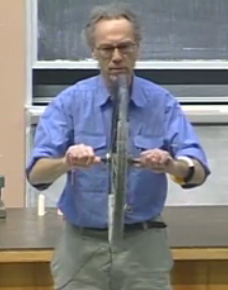
\includegraphics[scale=0.75]{\pIImages/lec24_bicycle_wheel}
\end{center}

(The reasoning for $\tau = b F$ is touched upon briefly just after the first picture in lecture 25.)

If the professor then were to push \emph{his} right hand forwards, while pulling his left right hand inwards, and apply a torque like that for a short amount of time, clearly the wheel will start spinning, counterclockwise as seen from above, and if we let it go, it will keep spinning like that forever. The torque causes a change in angular momentum, $\Delta L = \tau \Delta t$.

Next, we torque it so that the professor's left hand moves up, and his right hand moves down. This causes a rotation along a different axis, such that it spins counterclockwise as seen from our point of view (the angular velocity and angular momentum vectors are out of the screen). Again, it rotates like that forever along that axis.

Now... We spin the wheel up (along the axis a bicycle wheel \emph{should} rotate!), such that the angular velocity points to our right. What happens when he torques the wheel now?

The intuitive answer is, of course, that the wheel keeps spinning (it couldn't simply stop due to an unspecified amount of torque during an unspecified time) as a bicycle wheel does, while also rotating about the axis that we torqued it in. Without friction/air drag, both these rotations would continue on forever.

This is not what happens, though. It \emph{cannot} happen, without some external torque applied forever! The reason is that the spin angular momentum is pointing towards our right, as the experiment begins. After the torque, the intuitive answer states that this spin angular momentum would be changing direction constantly! How can a vector change direction and rotate, without any external torque? It cannot! Something else must happen.

What does happen is rather bizarre, and perhaps the most nonintuitive thing in the entire course.

As an important note on notation. any time I use ``spin'' below, I am talking about the wheel spinning like a bicycle wheel is meant to do.\\
Any time I use ``rotate'', I am talking about rotating about a different axis; one that never happens when it is attached to an actual bicycle going in a straight line.

\begin{center}
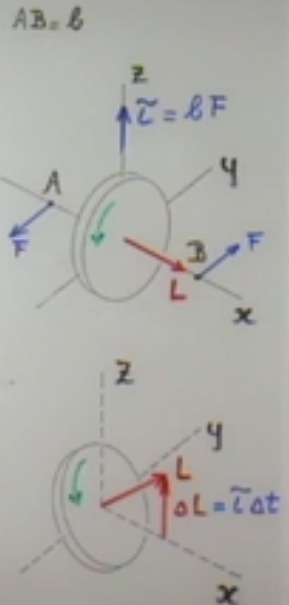
\includegraphics[scale=0.65]{\pIImages/lec24_wheel_directions}
\end{center}

As can be seen from this picture, which describes this exact situation, the torque is upwards. The spin angular momentum will ``follow'' this torque, and \emph{tilt the wheel} so that the angular spin momentum vector gets closer to the initial position of the torque.\\
That might not sound so strange, unless you keep the conditions in mind: the professor is doing a forwards/backwards push/pull on each side of the wheel, respectively, and instead of turning in the horizontal plane, it \emph{tilts} to the side! This is something that perhaps must be seen to be believed.

It is, of course, possible to predict what will happen, when we take what we know about physics into account. One very helpful thing to remember is that the spin angular momentum vector will always ``chase'' the torque vector. In this case, the torque is upwards, while the spin angular momentum is initially towards the right. In this situation, as we have seen, the wheel tilts such that the spin angular momentum is now pointing slightly upwards, as well.\\
When we reverse the torque, so the torque is downwards, the wheel tilts in the other direction.

What if the professor were to left his right hand up, and move his left hand down? Well, the spin angular momentum is towards the right to begin with. The torque, found as $\vec{r} \times \vec{F}$, now points either towards the blackboard (into the screen), or towards the audience (out of the screen). The wheel will now rotate as we would have expected it to rotate above. When the force along the moment arm is upwards, the wheel rotates so that the right axle (as we see it) points towards the audience.

The professor then demonstrates this by sitting a a stool that is free to rotate, while applying torque as mentioned above. The result is that as long as he keeps applying that force, the stool spins. As soon as he stops, the stool stops; if he torques in the opposite direction, the stool rotates in the opposite direction.\\
This principle can also be applied in space -- many satellites have ``reaction wheels'' that can be used to rotate the satellite, e.g. to keep it pointed in a certain direction.

This slower rotation, that the wheel experiences when exposed to a torque, is called \emph{precession}.

\subsection{Precession of a bicycle wheel on a string}

Next, we change the experiment up a bit. Instead of holding the wheel, we attach a rope to the end of one axis, and one axis only, such that gravity causes a rather strong torque on the wheel, that wants to rotate it downwards (so that it can fall down and simply hang there). That is of course exactly what will happen -- as long as the wheel is not spinning.

Here's what the setup looks like:

\begin{center}
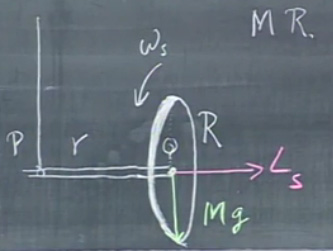
\includegraphics[scale=0.7]{\pIImages/lec24_wheel_gravity}
\end{center}

The thicker part of the wheel is towards the viewer.

The length of the axle is little $r$, while capital $R$ is the radius of the bicycle wheel. It is attached to the rope at point P.\\
As the wheel spins, with angular velocity $\omega_s$ (s for spin; we will soon see why a subscript is needed), it has spin angular momentum $L_s$ towards the right, as shown.\\
Gravity acts on the wheel's center of mass, which is approximately at the center of the wheel. Therefore, there is a torque relative to the center point Q, $\tau_Q = (\vec{r} \times \vec{g}) M = r M g$, given that there is a right angle between the moment arm (the axle $r$) and the force.

The direction of this torque is into the blackboard.\\
Unlike the previous situation, in ``outer space'', there \emph{is} now an external torque, due to gravity, that will act on the wheel forever. Since that torque vector is directed into the blackboard, what will happen is that, again, the spin angular momentum vector will ``chase'' that torque. The wheel will keep spinning, but also rotate (precess) \emph{counterclockwise}, as seen from above.

The torque is also changing, since the direction of the axle is constantly changing! It will change in such a way that there is indeed a counterclockwise precession; that is easy to convince oneself of by using the right-hand rule, especially if you use the entire right arm.\\
Point the right arm along the initial spin angular momentum vector, i.e. straight towards the right. Curl your fingers along the torque, exactly perpendicular, downwards (since gravity acts exactly downwards). Your right thumb now points ``forwards'', which is how the wheel will rotate.\\
A small amount later in time, the spin angular momentum will have chased the torque a bit in that direction, and so you need to rotate your entire right arm a bit forwards. Gravity is still straight down, but the new torque vector is slightly rotated compared to the first, so the spin angular momentum vector will never catch up, and the will will keep precessing (in the absence of losses; in reality, it will of course eventually fall down).

So how in the world can the wheel just stay up like that? Gravity acts on it, so it must fall -- $\displaystyle a_{cm} = \frac{F_{ext}}{m}$!\\
Well, no -- there is a string tension in the problem! The net force upwards/downwards on the system is zero -- the string tension equals $M g$, so no downwards acceleration of the center of mass is necessary!\\
So there is no net force on the object. There \emph{is} a net torque, however! This string tension does \emph{not} cancel out the torque due to gravity! The reason is that the tension has no moment arm! It acts through the point P, so it cannot contribute to torque about that point. The wheel's center of mass is located $r$ away from that point, so there is a torque $r M g$ due to gravity, as we saw above.

We can calculate the precession frequency of the wheel. The result is

\begin{equation}
\omega_{pr} = \frac{\tau}{L_s} = \frac{r M g}{I_Q \omega_s}
\end{equation}

The derivation for this is in the book: chapter 22, page 22-4 and forwards.

This is now why we used the subscript on $\omega$ previously. $\omega_s$ is the angular velocity of the spin, while $\omega_pr$ is the angular frequency of the precession -- which is a much, much smaller value. The wheel will spin at several rotations per second, while it will take the wheel about 10 seconds to complete one rotation due to the precession.\\
Note that this equation is also valid as long as the spin angular momentum is way, way larger than the angular momentum due to the ``orbital'' motion about point P (the rope). The total angular momentum of the system is $L_s$ plus the component due to the orbital motion, $I_P \omega_{pr}$ (where we have not calculated $I_P$).\\
The equation holds while the wheels spins quickly, but it predicts a precession frequency that goes to infinity as the wheel's spin slows down, which clearly doesn't make sense.

This result does make sense, though. If we increase the torque, the precession frequency will also increase. That makes some sense, since the torque is trying to ``win'' over the spin angular momentum, and force it to change to follow the torque. The stronger the torque, the easier it has to do this, and make the wheel rotate/precess.\\
On the other hand, the faster the wheel spins, the harder it is to precess. That also makes sense, for the same reason. The same happens as the moment of inertia along the spin axis increases, which also makes it tougher to attempt to change the spin angular momentum.

We can attempt to calculate the period of the precession. Using the above equation, we can use $r = 17$ cm, the length of the axle; $R = 29$ cm, the radius of the bicycle wheel; $f = 5$ Hz (approximate spin frequency of the wheel) so that $\omega_s = 2 \pi f_s = 10 \pi$ rad/s. With these numbers, we find

\begin{equation}
\omega_{pr} = \frac{r M g}{M R^2 \omega_s} = \frac{r g}{2 \pi f_s R^2} \approx \SI{0.631}{rad/s}
\end{equation}

The period is as always $T_{pr} = \frac{2 \pi}{\omega_{pr}} \approx \SI{10}{s}$. So the wheel will spin with at about 5 turns per second (300 rpm), and rotate due to precession with about one turn per ten seconds.\\
This is then demonstrated, in one of the more interesting demonstrations of the course so far.

Finally, the last lecture segment demonstrates a toy gyroscope, and a 3-axis gimbal gyroscope; on this last one, the spinning disk is mounted such that external forces do not cause a torque on the spinning disk, but rather, it is mounted such that the frames it is mounted in will rotate instead. Therefore, the spin angular momentum vector is always pointing in one direction, no matter how you turn the outer part of the gyroscope. This is used in gyrocompasses, and inertial guidance systems, etc.
